\icode{O-MM-SU-261001}
\lkf{物理模型：}一个质量为\(m_1\)的球\(A\)以\(v_0\)的速度正心碰撞静止的球\(B\)，如图所示。
	\begin{figure}[htbp]
		\centering
		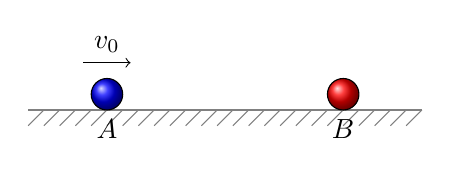
\begin{tikzpicture}
			\draw[gray] (0,0)--(5,0);
			\foreach \x in {0,.2,...,4.8}
				\draw[gray] (\x,-.2)--++(.2,.2);
			\shadedraw[ball color=blue] (1,.2) circle(.2);
			\shadedraw[ball color=red] (4,.2) circle(.2);
			\foreach \x/\y/\c in {1/0/A,4/0/B}
				\node at(\x,\y) [below]{\(\c\)};
			\draw[->] (.7,.6)--node[above]{\(v_0\)}(1.3,.6);
		\end{tikzpicture}
	\end{figure}
	碰后\(A\)、\(B\)的速度分别为\(v_1\)、\(v_2\)

	{\fangsong \(A\)、\(B\)碰撞动量守恒，可得
	\[
		m_1v_0 = m_1v_1 + m_2v_2\Longrightarrow v_2 = \frac{m_1}{m_2}(v_0 - v_1)
	\]
	碰后损失的动能记作\(\Delta E_{k\text{损}}\)，则
	\[
		\begin{aligned}
			\Delta E_{k\text{损}}&=\frac{1}{2}m_1v_0^2 - \frac{1}{2}m_1v_1^2 - \frac{1}{2}m_2v_2^2\\
			&= \frac{1}{2}m_1v_0^2 - \frac{1}{2}m_1v_1 - \frac{1}{2}m_2[\frac{m_1}{m_2}(v_0 - v_1)]^2\\
			&= -\frac{m_1}{2m_2}(v_1 - v_0)[(m_1 + m_2)v_1 - (m_1 - m_2)v_0]\\
			&= \frac{m_1}{2m_2}[ -(m_1 + m_2)\cdot v_1^2 + 2m_1v_0\cdot v_1 -(m_1 - m_2)v_0^2]
		\end{aligned}
	\]
	用\(B\)的速度\(v_2\)表示动能损失，则
	\[
		\begin{aligned}
			\Delta E_{k\text{损}}&=\frac{1}{2}m_1v_0^2 - \frac{1}{2}m_1v_1^2 - \frac{1}{2}m_2v_2^2\\
			&= \frac{1}{2}m_1v_0^2 - \frac{1}{2}m_1(\frac{m_1v_0 - m_2v_2}{m_1})^2 - \frac{1}{2}m_2v_2^2\\
			&=- m_2v_2[(\frac{m_1 + m_2}{2m_1}v_2 - v_0)]\\
			&=- \frac{m_2(m_1 + m_2)}{2m_1}\cdot v_2^2 + m_2v_0\cdot v_2
		\end{aligned}
	\]
	当\(AB\)共速时，\(\Delta E_{k\text{损}}\)最大
	\[
		\Delta E_k = \frac{1}{2}\frac{m_1m_2}{m_1 + m_2}v_0^2
	\]
	式中\(\frac{m_1m_2}{m_1 + m_2}\)叫做约化质量。
	}
	
	\begin{minipage}[c]{.45\textwidth}
		\centering
		\begin{tikzpicture}
			\draw[blue,->] (-2,0)--(4,0)node[below]{\(v_1\)};
			\draw[blue,->] (0,-1)--(0,4)node[right]{\(\Delta E_{k\text{损}}\)};
			\node[blue] at(.2,.2){\(O\)};
			\draw[orange] (-1,0) parabola bend(1,3) (3,0);
			\node at(3,0) [below]{\(v_0\)};
			\node at(-1,0) [below]{\(\frac{(m_1 - m_2)v_0}{m_1 + m_2}\)};
			\draw[dashed] (0,3)--(1,3)--(1,0)node[below]{\(\frac{m_1v_0}{m_1 + m_2}\)};
			\node at(0,3)[left]{\(\frac{1}{2}\frac{m_1m_2}{m_1 + m_2}v_0^2\)};
		\end{tikzpicture}
	\end{minipage}
	\begin{minipage}[c]{.49\textwidth}
		\centering
		\begin{tikzpicture}
			\draw[blue,->] (-1,0)--(5,0)node[below]{\(v_2\)};
			\draw[blue,->] (0,-1)--(0,4)node[right]{\(\Delta E_{k\text{损}}\)};
			\node[blue] at(-.2,-.2){\(O\)};
			\draw[teal] (0,0) parabola bend(2,3) (4,0);
			\node at(4,0) [below]{\(\frac{2m_1v_0}{m_1 + m_2}\)};
			\draw[dashed] (0,3)--(2,3)--(2,0)node[below]{\(\frac{m_1v_0}{m_1 + m_2}\)};
			\node at(0,3)[left]{\(\frac{1}{2}\frac{m_1m_2}{m_1 + m_2}v_0^2\)};
		\end{tikzpicture}
	\end{minipage}